\documentclass[a4paper,
               %boxit,
               %titlepage,   % separate title page
               %refpage      % separate references
              ]{jacow}
%
% CHANGE SEQUENCE OF GRAPHICS EXTENSION TO BE EMBEDDED
% ----------------------------------------------------
% test for XeTeX where the sequence is by default eps-> pdf, jpg, png, pdf, ...
%    and the JACoW template provides JACpic2v3.eps and JACpic2v3.jpg which
%    might generates errors, therefore PNG and JPG first
%
\makeatletter%
	\ifboolexpr{bool{xetex}}
	 {\renewcommand{\Gin@extensions}{.pdf,%
	                    .png,.jpg,.bmp,.pict,.tif,.psd,.mac,.sga,.tga,.gif,%
	                    .eps,.ps,%
	                    }}{}
\makeatother

% CHECK FOR XeTeX/LuaTeX BEFORE DEFINING AN INPUT ENCODING
% --------------------------------------------------------
%   utf8  is default for XeTeX/LuaTeX 
%   utf8  in LaTeX only realises a small portion of codes
%
\ifboolexpr{bool{xetex} or bool{luatex}} % test for XeTeX/LuaTeX
 {}                                      % input encoding is utf8 by default
 {\usepackage[utf8]{inputenc}}           % switch to utf8

\usepackage[USenglish]{babel}			 

\usepackage[final]{pdfpages}
\usepackage{multirow}
\usepackage{ragged2e}

%
% if BibLaTeX is used
%
\ifboolexpr{bool{jacowbiblatex}}%
 {%
  \addbibresource{jacow-test.bib}
  \addbibresource{biblatex-examples.bib}
 }{}
\listfiles

%
% command for typesetting a \section like word
%
\newcommand\SEC[1]{\textbf{\uppercase{#1}}}

%%
%%   Lengths for the spaces in the title
%%   \setlength\titleblockstartskip{..}  %before title, default 3pt
%%   \setlength\titleblockmiddleskip{..} %between title + author, default 1em
%%   \setlength\titleblockendskip{..}    %afterauthor, default 1em

%\copyrightspace %default 1cm. arbitrary size with e.g. \copyrightspace[2cm]

% testing to fill the copyright space
%\usepackage{eso-pic}
%\AddToShipoutPictureFG*{\AtTextLowerLeft{\textcolor{red}{COPYRIGHTSPACE}}}

\begin{document}

\title{Input Signal Generation for Barrier Bucket RF Systems at GSI\thanks{Work supported by BMBF and GSI}}

\author{J. Harzheim\thanks{harzheim@temf.tu-darmstadt.de}, D. Domont-Yankulova, K. Groß, H. Klingbeil\textsuperscript{1} TU Darmstadt, Darmstadt, Germany
	\\
	M.  Frey, GSI, Darmstadt, Germany
	\\
	\textsuperscript{1} also at GSI, Darmstadt, Germany}
	
\maketitle

%
\begin{abstract}
	 At GSI, Barrier Bucket RF systems are currently designed for the SIS 100 synchrotron (part of the future accelerator 
	 facility FAIR) \cite{FAIR} and the Experimental Storage Ring (ESR) \cite{Demo_BB_ESR}. The purpose of these systems is 
	 to provide pulsed voltages (Fig.~1) at the cavity gap in order to facilitate several longitudinal bunch manipulations.	 
	 %To achieve the high quality signals required for the future FAIR experiments, 
	 To achieve the desired signal quality, the design and matching of the different components as well as a proper mathematical modeling
	 of the system is needed. This contribution focuses on the system identification and modeling for the ESR Barrier Bucket system to
	 calculate the input signal for the requested output voltage.
	 In a first step, the system is modeled using a linear model, which is sufficient up to gap voltages of 550\,V. 
	 At higher amplitudes, nonlinear effects begin to occur, reducing the output signal quality. Therefore, the linear model is extended to a Hammerstein 
	 model which consists of a static nonlinearity followed by the linear part. Measurement results show that this approach significantly improves the 
	 signal quality at high amplitudes.
	 
\end{abstract}

%----------------------------------------------------------------
\section{Introduction} \vspace*{0.5em} 
	 
	 %Barrier Bucket (BB) in general (see IPAC 2016)
	 Barrier Bucket (BB) systems enable a large variety of longitudinal beam manipulations in synchrotrons and storage rings  (e.g. [3-5]) by using %\cite{BB_Fermilab}, \cite{BB_dynamics}, \cite{Buch_HK}) by using
	 pulsed gap voltages (see Fig.~1). If the repetition frequency of the voltage pulse equals the revolution frequency of the 
	 beam, this voltage pulse forms a stationary potential barrier in phase space. When both frequencies differ, the barrier is moving in phase space (``moving barriers'', e.g. [6-8]). %\cite{BB_dynamics_synchrotron}, \cite{MOV_B2}, \cite{Mov_B1}).
	 Particles moving in the ring can be confined between two barriers, allowing variable bucket lengths and applications like bunch merging, compression or 
	 decompression.\\
	 In order to deliver high intensity beams of high quality, as needed for the planned experiments at FAIR, requirements on the gap voltage 
	 qualities for acceleration and Barrier Bucket operation are very high as well. Hence, a lot of effort needs to be spent on the design of the system, but
	 also on the proper mathematical modeling in order to be able to calculate the accurate input signal.
	 At GSI, a prototype setup of the future ESR BB system is currently under investigation [9-10]. The three main components are a broadband cavity filled with %\cite{Paper_Frey}, \cite{Paper_Gross}. The three main components are a broadband cavity filled with 
	 Magnetic Alloy ring cores [11-13], a solid state amplifier (amplifier research 1000A225) and a signal generator (Keysight 3600A series 2-channel AWG).  %\cite{RK_2}, \cite{RK_1}, \cite{Harzheim:IPAC2016-MOPMW002}, a solid state amplifier (amplifier research 1000A225) and a signal generator (Keysight 3600A series 2-channel AWG). 
	 A simplified setup of the system is shown in Fig.~\ref{Modellierung}.	 

	 %--> important, components need properties whose modeling can be handled
	 
	 %A procedure to generate the input signal based on the dynamic properties in the linear region of the system has been developed 
	 %and tested at a prototype system. It was shown that this method is able to generate s
	 %ingle sine gap signals of high quality in a wide voltage range. As linearity can only be assumed up to a certain magnitude, 
	 %nonlinear effects limit the quality of the output signal at very high input levels. 
	 %An approach to overcome this limit is to extend the input signal calculation to a nonlinear model of the system.
	 


	  %In this contribution, the current model of the ESR Barrier Bucket System and the corresponding predistortion method for the input signal
	  %are presented %periodic operation 
	  
	  %is presented  to calculate the required input signal for linear operation is presented and experimental results at a prototype system are 
	  %shown. Additionally, first results in the 
	 %nonlinear region are presented.	 
	 % figure: Einzelsinus mit T_BB und T_rep etc.
	
	
	\section{Signal requirements}
		 %\begin{minipage}{0.32\textwidth}
	%Lieber in eine Tabelle??????
	
	For the ESR BB system, single-sine voltage pulses with a repetition frequency $f_{rep}$ of 900\,kHz and a BB frequency $f_{BB}$ of 5\,MHz are required 
	(see Fig.~\ref{bb_signal}). The desired amplitude $\hat{U}_{BB}$ of the pulse is 1\,kV. As voltages aside the pulse (so called ``ringing'') can 
	lead to microbunching, the ringing must	stay in $\pm$2,5\% of $\hat{U}_{BB}$. Additionally, the difference between positive and negative half cycle 
	should be in the range of $\pm$5\% of $\hat{U}_{BB}$. The values were taken from \cite{SIS100_spec}.
	
	 \includegraphics[scale=0.42]{WEPVA047f1.eps}
	   \captionof{figure}{Desired output gap voltage.}
	  \label{bb_signal}
	  
	 \section{Linear region}
	For sufficiently small input signals, most systems can be described by a linearization around the system's operating point.
	In this linear region, the relation between the input signal $\underline{U}_{AWG}(\omega)=\underline{U}_{in}(\omega)$ and the output signal 
	$\underline{U}_{out}(\omega)$ is given by the system's frequency response $\underline{H}(\omega)$:
	\begin{equation}
	 \underline{U}_{out}(\omega)=\underline{U}_{in}(\omega)\cdot\underline{H}(\omega).
	 \label{H}
	\end{equation}
	For the prototype setup, the input signal is the signal created by the signal generator and the output signal is the voltage measured at the cavity gap.
	
	%\vspace{0.3cm}
	%\begin{figure}
	% \begin{center}
	% \includegraphics[scale=0.2]{Messaufbau.eps}
	%  \label{Messaufbau}
	%  %\vspace{-1cm}
	%  \captionof{figure}{Measurement setup to determine the system's transfer function} 
	% \end{center}
	%\end{figure}
	
	In order to determine the input signal of the system, the frequency response has to be measured. %This was done at the ESR BB prototype setup shown in Figure 2. 
	For the measurement, a small signal frequency sweep from 10\,kHz to 80\,MHz was applied to the system. The sweep was performed sufficiently slowly
	(e.g.~25 minutes) to ensure steady state conditions. 
	
	\begin{figure*}[!tbh]
	\centering
	\includegraphics*[width=0.7\textwidth]{WEPVA047f2.eps}
	\caption{Hammerstein modeling of the ESR BB prototype system.}
	\label{Modellierung}
%    	\vspace*{-\baselineskip}
	\end{figure*}
	%lalalalala
	
	A two channel AWG was used as a signal generator with channel 1	connected to the RF power amplifier and channel~2 connected to the oscilloscope to measure 
	the undistorted input signal $\underline{U}_{in}$. The output signal $\underline{U}_{out}$ (voltage at the cavity gap) was measured using the 
	same oscilloscope. This way, the difference in amplitude and phase between input and output signal can be observed at each frequency point. 
	$\underline{H}(\omega)$ can be calculated from measurement data
	by
	\begin{equation}
	 \underline{H}(\omega)=\frac{\underline{U}_{out}(\omega)}{\underline{U}_{in}(\omega)}.
	\end{equation}
	%\end{minipage}
	The measured amplitude response of the system is shown in Fig.~\ref{H_ESR}.
	
	\begin{figure}[b]
	 \begin{center}
	  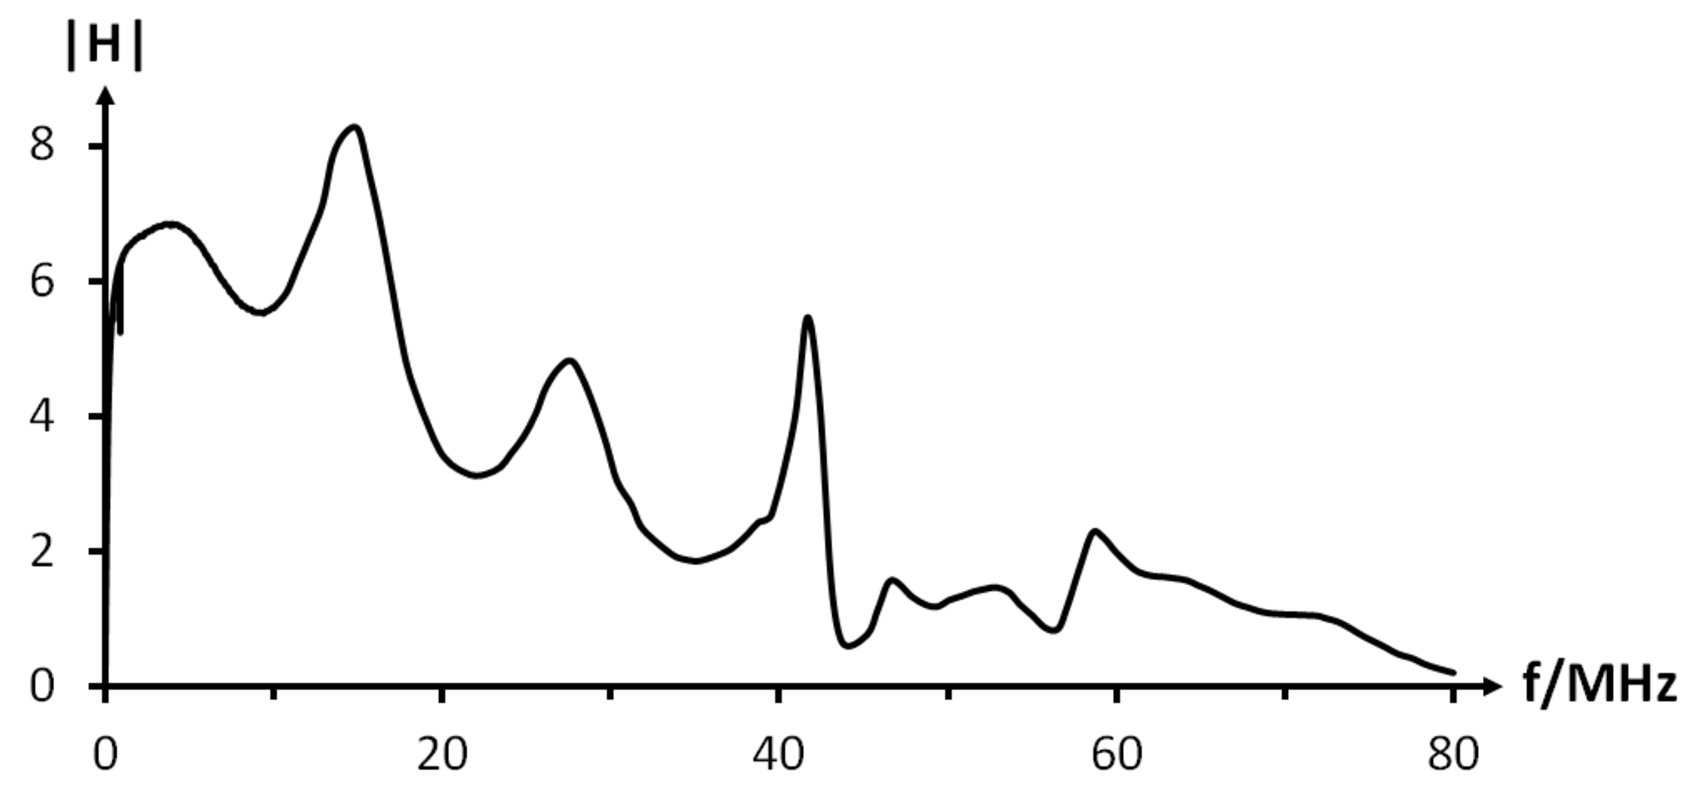
\includegraphics[scale=0.27]{WEPVA047f3.eps}
	  %\vspace{-1cm}
	  \captionof{figure}{Measured amplitude response of the ESR BB system.} 
	  \label{H_ESR}
	  \vspace*{-\baselineskip}
	 \end{center}
	 	%\hspace{-1cm}
	\end{figure}	

	
	For periodic BB operation (see Fig.~1), the desired output signal during one period $T_{rep}$ is defined as
	\begin{equation}
	 U_{out}(t)=\begin{cases}
	             -\hat{U}\cdot \text{sin}\left(\frac{2\pi}{T_{BB}}t\right) \quad \text{for} \quad -\frac{T_{BB}}{2}<t<\frac{T_{BB}}{2} \\
	             0 \qquad \qquad \qquad \text{else}
	            \end{cases}.
	\end{equation}
	Using Fourier decomposition \cite{gross}, the signal can be described by 
	\begin{equation}
	  U_{out}(t)=\sum \limits_{n=1}^\infty b_{n,\text{out}}\cdot \text{sin}(n\omega_{rep}t)
	  \label{U_out}
	\end{equation}
	with the Fourier coefficients
	\begin{equation}
	  b_{n, \text{out}}=\hat{U}\frac{T_{BB}}{T_{rep}}\left[\text{si}\left(\pi\left[n\frac{T_{BB}}{T_{rep}}+1\right]\right)-\text{si}\left(\pi\left[n\frac{T_{BB}}{T_{rep}}-1\right]\right)\right].
	\end{equation}	
	Due to linearity, the input signal for the linear region of the system can be derived from Eq.~\eqref{H} and \eqref{U_out}:
	\begin{equation}
	  U_{in}(t)=\sum \limits_{n=1}^\infty \frac{b_{n,\text{out}}}{|\underline{H}(n\omega_{rep})|}\cdot \text{sin}\left(n\omega_{rep}t-\text{arg}[\underline{H}(n\omega_{rep})]\right).
	  \label{VV_lin}
	\end{equation}

	%\begin{minipage}{0.15\textwidth}
	Measurements at the prototype system showed that the linear method can	produce signals of sufficiently high quality up to gap voltages of about 550\,V peak. A measurement of the predistorted input signal and 
	the corresponding output signal for \mbox{$f_{BB}=5\,\text{MHz}$} and \mbox{$f_{rep}=900\,\text{kHz}$} is shown in Fig.~4. 
			
	\begin{figure}[!h]
	\vspace{-0.5\baselineskip}
	\begin{center}
	 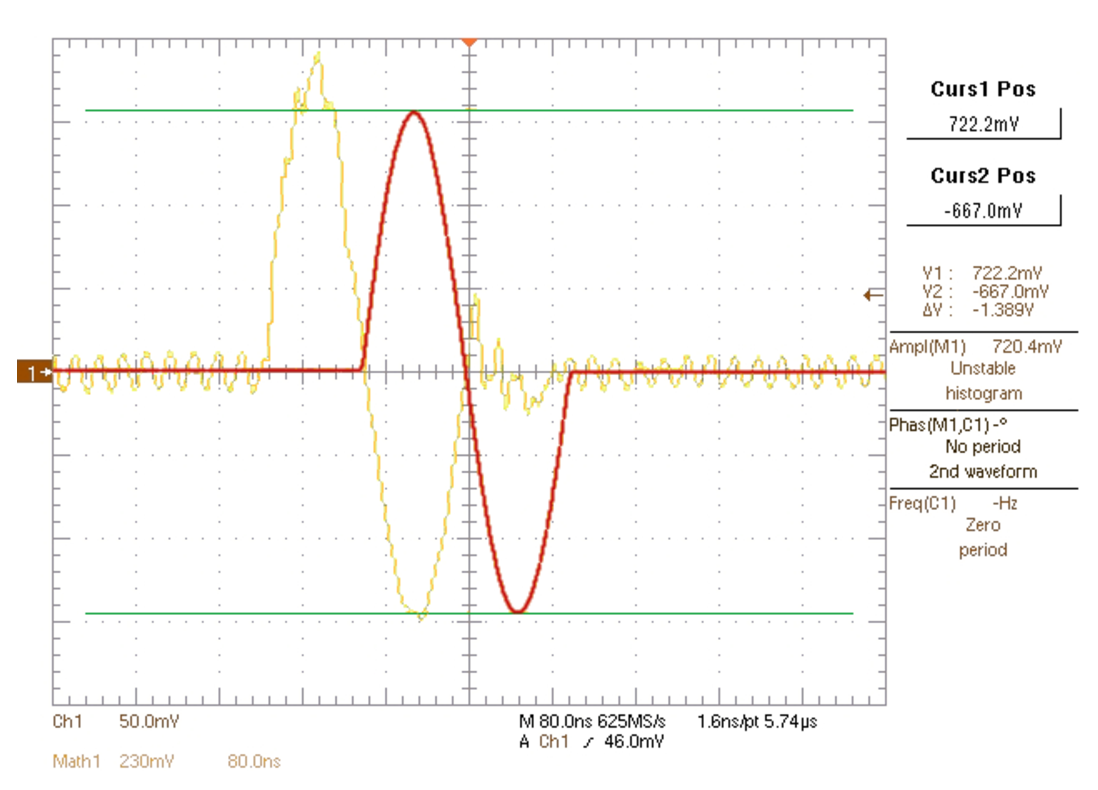
\includegraphics[scale=0.42]{WEPVA047f4.eps}
	  \label{Signal}
	  %\vspace{-1.5cm}
	  \captionof{figure}{Measured input and output signal in the linear region ($\hat{U}=520\,V$).}	  	 
	\end{center}
	\vspace{-\baselineskip}
	\end{figure}
	
	%\end{minipage}
	%\begin{minipage}{0.01\textwidth}
	 %\hspace{0.4cm}
	%\end{minipage}
	%\begin{minipage}{0.28\textwidth}
	%\begin{minipage}{0.28\textwidth}
	%\vspace{-1cm}
	
	\section{Nonlinear Approach}			
	%\newpage
	To improve signal quality at high amplitudes, nonlinear effects have to be taken into account. As expected, measurements taken with the solid state amplifier
	showed that the output nonlinearly depends on the amplitude of the input signal. Therefore, the amplifier is modeled as a nonlinear voltage-controlled
	voltage source followed by an unknown output impedance (Fig.~2). For the cavity, only linear effects
	are expected that determine the dynamic behaviour, as the magnetic field strength inside the MA ring cores of the cavity is far below ($\le 5\%$) 
	saturation field strength \cite{VV_JH}. Presuming ideal matching between the signal generator and the amplifier input, it seems reasonable to hypothesize a Hammerstein
	system (a static nonlinearity followed by a linear system, e.g. [17-19]) as a simplified nonlinear model for the system %\cite{Buch_Nonl}, \cite{Ham1},  \cite{Ham2}) as a simplified nonlinear model for the system 
	(see Fig.~\ref{Modellierung}).
	
	To characterize the static nonlinearity, a power series ansatz was chosen. With an $N$th-order power series, the relation between $U_{in}$ and $U_?$
	can be described as
	
	\begin{equation}
	 U_?(t)=\sum_{n=1}^N a_n \left[ U_{in}(t) \right]^n.
	 \label{Potenzreihe}
	\end{equation}
	
	Since $U_?(t)$ can't be externally measured, $\underline{U}_?(\omega)$ was calculated in the frequency domain from the measured output voltage $U_{out}(t)$ 
	using the frequency response measured afore:	
	\begin{equation}
	 \underline{U}_?(\omega)=\underline{U}_{out}(\omega)\cdot \underline{H}^{-1}(\omega).
	 \label{inv}
	\end{equation}	
	Afterwards, $\underline{U}_?(\omega)$  is transformed back into time domain. 	
	%\newpage
	The estimation of the coefficients $a_n$ in Eq.~\eqref{Potenzreihe} 
	can be treated as a linear optimization problem by comparing single samples $U_{?,i}=U_?(i\cdot\Delta t)$ with the corresponding samples of the input 
	signal $U_{in,i}=U_{in}(i\cdot\Delta t)$. 
	For an input signal of $M$ samples and a power series of order $N$, Eq.~\eqref{Potenzreihe} yields
	\begin{equation}
	 \left( 
	 \begin{matrix}
	  U_{in,1} & U_{in,1}^2 & \dots & U_{in,1}^N \\
	  U_{in,2} & U_{in,2}^2 & \dots & U_{in,2}^N \\
	  \vdots & \vdots & \ddots & \vdots \\
	  U_{in,M} & U_{in,M}^2 & \dots & U_{in,M}^N \\
	 \end{matrix}
	\right)
	\cdot
	\left(
	\begin{matrix}
	 a_1 \\
	 a_2 \\
	 \vdots \\
	 a_N \\	 
	\end{matrix}
	\right) 
	= \left( 
	\begin{matrix}
	 U_{?,1} \\
	 U_{?,2} \\
	 \vdots \\
	 U_{?,M} \\	 
	\end{matrix}
	\right).
	\label{lgs}
	\end{equation}

	
	As usually $M>N$ applies, Eq.~\eqref{lgs} is overdetermined and was solved using a least-square algorithm. Linearly predistorted signals according to 
	Eq.~\eqref{VV_lin} with different amplitudes were used for $U_{in}(t)$. Figure 5 shows a comparison of $U_{in}(t)$ and $U_?(t)$ calculated with 
	Eq.~\eqref{inv}.		
	
	\begin{figure}[!h]
	\vspace*{-.5\baselineskip}
	 \begin{center}
	  \includegraphics[scale=0.3]{WEPVA047f5.eps}
	 \label{Vergleich1}
	 %\vspace{-1cm}
	 \captionof{figure}{Comparison of $U_{in}$ and $U_?$ for $\hat{U}_{in}=280~\text{mV}_\text{pp}$.} %$U_in=280\textmd{mV}_\textmd{pp}}$}
	 \end{center}
	\vspace*{-\baselineskip}	 
	\end{figure}
	
	Measurements showed that best output qualities can be achieved with power series of 3rd or 4th order. The resulting 3rd order nonlinear characteristic 
	is shown in Fig.~6.
	\begin{figure}
	\vspace*{-.5\baselineskip}
	 \begin{center}
	  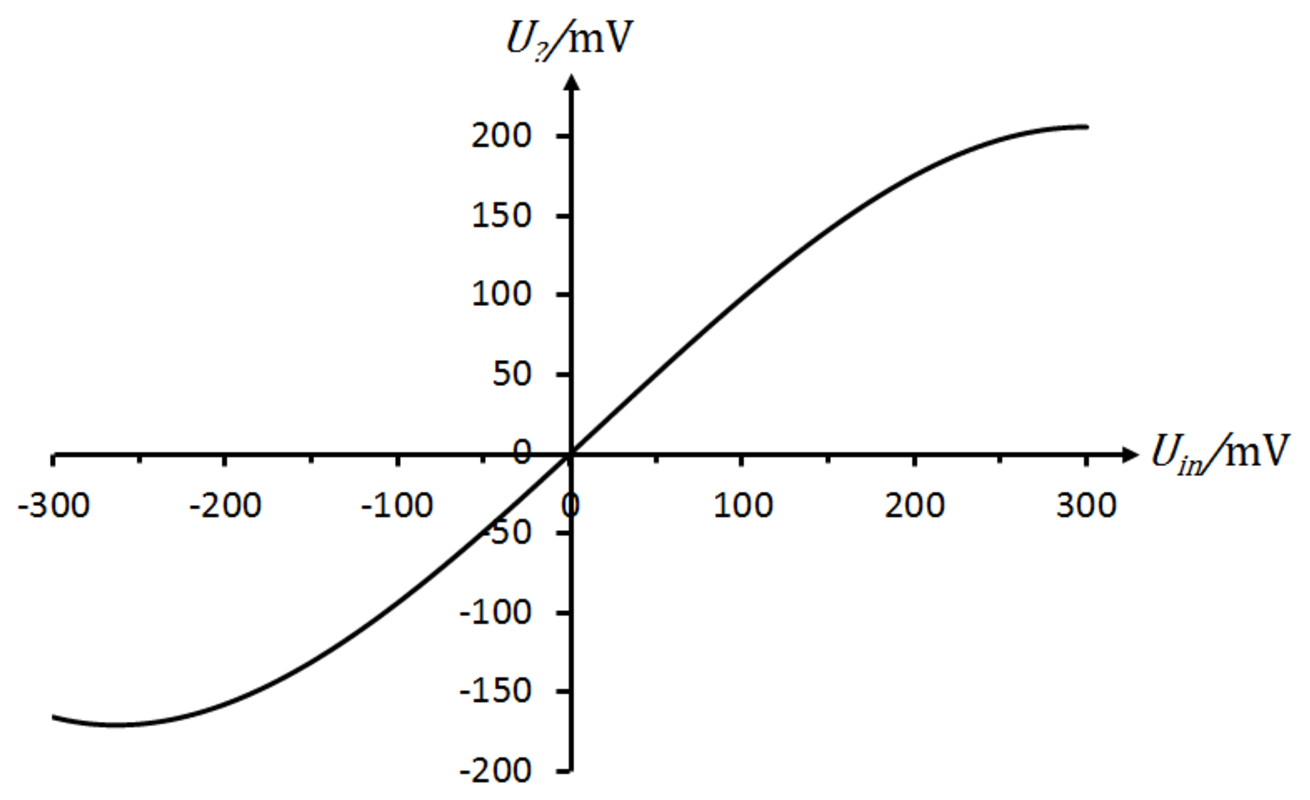
\includegraphics[scale=0.3]{WEPVA047f6.eps}
	 \label{Kennlinie}
	 %\vspace{-1cm}
	 \captionof{figure}{Measured 3rd order polynomial nonlinearity.}
	 \end{center}
	 \vspace*{-\baselineskip}
	\end{figure}

	Based on the measured characteristic, the inverse characteristic was computed and stored in form of a look-up table. To include the nonlinear
	part of the model in the input signal calculation, the signal calculated for the linear region according to Eq.~\eqref{VV_lin} is predistorted
	using the inverse characteristic of the look-up table. The resulting output signals are shown in Fig.~7.

	 The additional nonlinear predistortion obviously leads to a significant improvement of the output voltage quality. Ringing
	 can be reduced to below 1\% which fulfills the specification. The difference between positive and negative half-cycle is 7\% which is slightly 
	 outside the specification. However, all requirements can be satisfied when the output amplitude is reduced to 760\,V.
	 During the measurements it also became visible, that the positive half-cycle of the output voltage can't be increased much above 820\,V independent of the input
	 voltage. This might indicate that the pulse-power limit of the amplifier is reached. In that case, further increase of the amplitude for the given
	 system is not possible.
	 	
	\begin{figure}[h]
       \vspace*{-.5\baselineskip}
	\begin{center}
	%\vspace{-1cm}
	 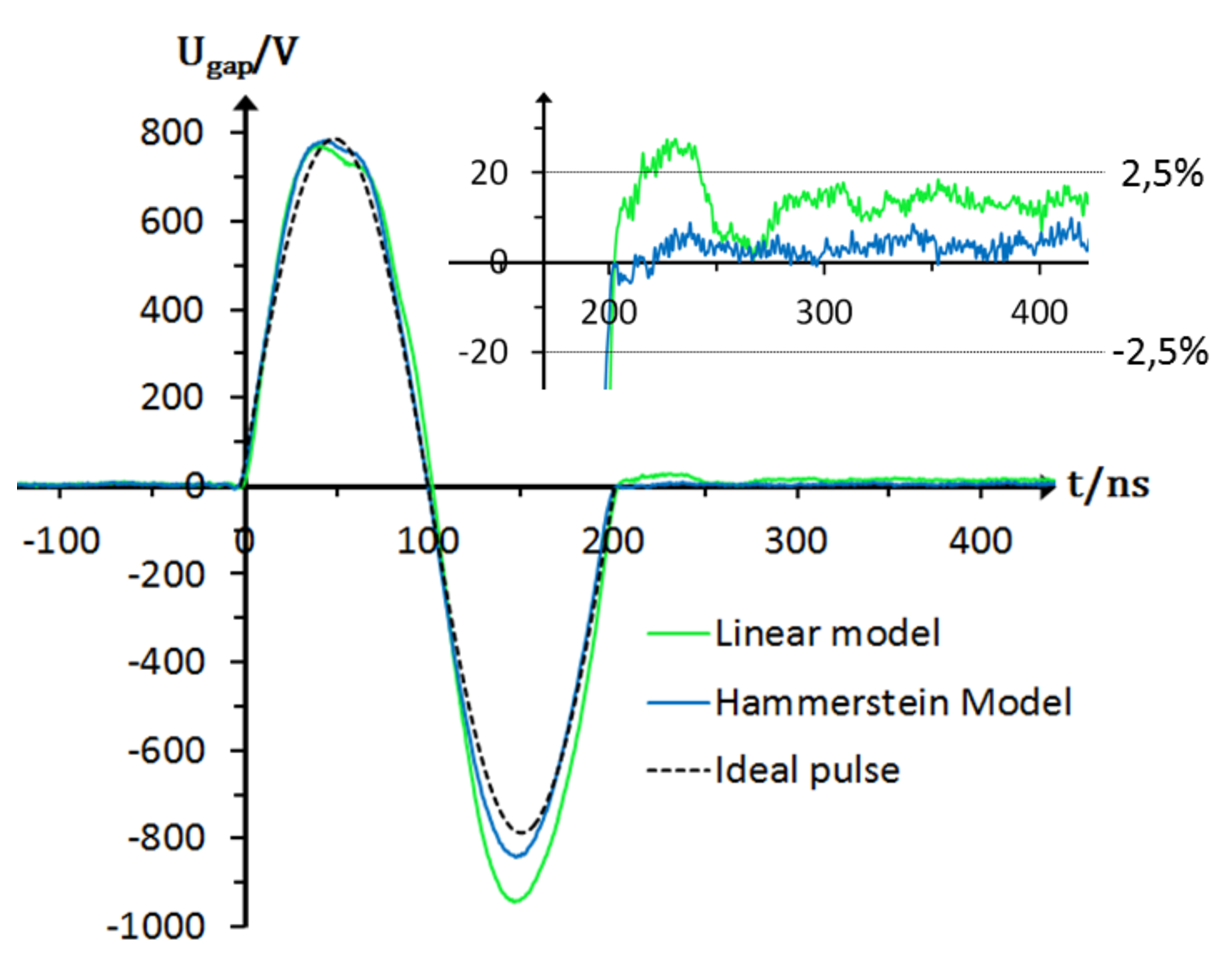
\includegraphics[scale=0.36]{WEPVA047f7.eps}
	 \label{Vergleich}
	 %\vspace{-0.2cm}
	 \captionof{figure}{Resulting voltages for linear and nonlinear predistortion for $\hat{U}=800\,V$.}
	 \end{center}	 
	 \vspace*{-\baselineskip}
	\end{figure} 
	
	%\begin{figure*}[!tbh]
	%\centering
	%\includegraphics*[width=0.7\textwidth]{Modelling.eps}
	%\caption{Hammerstein modeling of the ESR BB System}
	%\label{Modellierung}
%    	\vspace*{-\baselineskip}
	%\end{figure*}
	%lalalalala
	
	\section{Conclusion}
	Measurements at a BB prototype system showed that the current linear method is able to generate single sine gap signals of high quality in a wide voltage range. %A Hammerstein model was introduced to cope with nonlinear effects at high amplitudes.
	It was also shown that the assumption of a static nonlinearity in form of a 3rd order polynomial can significantly improve the gap signal quality at high amplitudes. 
	One possibility to further increase the output quality and amplitude could be to try different parametrizations for the estimation of the nonlinear characteristic or to
	use a more complex model. However, measurements indicate that the amplifier of the prototype system reaches its pulse-power limit at an output amplitude
	of about 800\,V. Therefore, a further increase of the output voltage might not be possible even with a more complex model.
	%Consequently, one future research emphasis will be the investigation and implementation of 
	%more powerful system identification algorithms to determine the nonlinearity more precisely. 

%----------------------------------------------------------------
\newpage

\iffalse  % only for "biblatex"
	\newpage
	\printbibliography

% "biblatex" is not used, go the "manual" way
\else

\begin{thebibliography}{99} % Use for 1-9 references

%\bibitem{accelconf-ref}
%	C. Petit-Jean-Genaz and J. Poole,
%	``JACoW, A service to the Accelerator Community,''
%	EPAC'04, Lucerne, July 2004, THZCH03,  p.~249,
%	\url{http://www.JACoW.org/e04/papers/THZCH03.PDF}
\bibitem{FAIR}
	H. H. Gutbrod \textit{et al.}, “FAIR - Baseline Technical Report, Volume 2, Accelerator and Scientific Infrastructure“,
	GSI, Darmstadt, Germany, September 2006.
			
\bibitem{Demo_BB_ESR}
	M. Steck \textit{et al.}, “Demonstration of Longitudinal Stacking in the ESR with Barrier Buckets and Stochastic Cooling“,
	in \textit{Proc. COOL 2011}, Alushta, Ukraine, September 2011, paper TUPS20, pp. 140-143.
	
\bibitem{BB_Fermilab}
	C. M. Bhat, “Applications of barrier bucket RF systems at Fermilab“,
	FNAL, Batavia IL, USA, Rep. FERMILAB-CONF-06-102-AD, March 2006.
	
		
\bibitem{BB_dynamics}
	C. M. Bhat, “Particle dynamics in storage rings with barrier rf systems“,
	\textit{Physical Review E}, vol.~55, no.~5, p.~5992, May 1997.

	
\bibitem{Buch_HK}
	H. Klingbeil, U. Laier and D. Lens, “Theoretical Foundations of Synchrotron and Storage Ring RF Systems“,
	Springer, Heidelberg, Germany, 2015.
	
\bibitem{BB_dynamics_synchrotron}
	C. M. Bhat, “Barrier rf systems in synchrotrons“,
	FNAL, Batavia IL, USA, Rep. FERMILAB-CONF-04-091-AD, 2004.
		
\bibitem{MOV_B2}
	O. Boine-Frankenheim, “RF barrier compression with space charge“,
	in \textit{Physical Review} ST Accel. Beams 13, 034202,
	Germany, March 2010.
	
\bibitem{Mov_B1}	
	M. Krestnikov \textit{et al.}, “Particle Accumulation Using Barrier Bucket RF System“,
	in \textit{Proc. COOL'09}, Lanzhou, China, 2009, paper TUM2MCIO02, pp. 67-70.
	
\bibitem{Paper_Frey}
	M. Frey, D. Domont-Yankulova, J. Harzheim, K. Groß and H. Klingbeil, “Prototype Results of the ESR Barrier Bucket System“,
	in \textit{Proc. IPAC'17}, Copenhagen, Denmark, May 2017, paper THPIK015, this conference.
	
\bibitem{Paper_Gross}
	K. Gross, D. Domont-Yankulova, M. Frey, J. Harzheim and H. Klingbeil, “Test Setup for Automated Barrier Bucket Signal Generation“,
	in \textit{Proc. IPAC'17}, Copenhagen, Denmark, May 2017, paper THPAB098, this conference.

	
%\bibitem{ring_core}
%	S. Jatta, “Umgebungseinfluss bei Messungen  mit MA-Ringkernen“,
%	GSI internal report,
%	GSI Darmstadt, Germany, 2013.
	
%\bibitem{vector_fitting}
%	B. Gustavsen a	B. Gustavsen and A. Semlyen, “A robust approach for system identification in the frequency domai“
%	in \textit{IEEE Trans. Power Delivery}, vol. 19, no. 3, pp. 1167-1173, July 2004.	
	
%\bibitem{vec_f1}
%	B. Gustavsen and A. Semlyen, “Enforcing passivity for admittance matrices approximated by rational functions“,
%	in \textit{IEEE Trans. Power Systems}, vol. 16, no. 1, pp. 97-104, February 2001.
	
%\bibitem{vec_f2}
%	B. Gustavsen, “Computer code for rational approximation of frequency dependent admittance matrices“, 
%	in \textit{IEEE Trans. Power Delivery}, vol. 17, no. 4, pp. 1093-1098, October 2002.
	
\bibitem{RK_2}
	C. Ohmori \textit{et al.}, “A wideband RF cavity for JHF synchrotrons“, 
	in \textit{Proc. Particle Accelerator Conference 1997}, Vancouver, BC, Canada, May 1997, pp. 2995-2997.

\bibitem{RK_1}
	T. Trupp, “NANOPERM® Broad Band Magnetic Alloy Cores for Synchrotron RF Systems“,
	in \textit{Proc. IPAC2014}, Dresden, Germany, 2004, paper MOPRO016, pp. 95-98.	
	
\bibitem{Harzheim:IPAC2016-MOPMW002}
	J. Harzheim, D. Domont-Yankulova, M. Frey, H. Klingbeil, and R. Königstein,
	“Modeling and Simulation of Broadband RF Cavities in PSpice“,
	in \textit{Proc. IPAC’16},
	Busan, South Corea, May 2016, 
	paper MOPMW002, pp. 392--395.	
	
\bibitem{SIS100_spec}
	GSI PBRF Department, “Detailed Specification of the SIS100 Barrier Bucket System for FAIR“,
	GSI internal report, GSI Darmstadt, Germany, August 2016.
   
%\bibitem{HESR_BB}
%	R. Stassen \textit{et al.}, “The HESR RF-system and tests in COSY“,
%	in \textit{Proc. EPAC08}, Genoa, Italy, 2008, paper MOPC125, pp. 361-363.
	
\bibitem{gross}
	S. Jatta and K. Gross, “Spectrum of the BB signal at different periodicities“,
	GSI internal report, GSI Darmstadt, Germany, November 2013. %\newline	
	
\bibitem{VV_JH}
	J.~Harzheim, “Zusammenfassung nichtlineare Vorverzerrung“,
	GSI internal report, GSI Darmstadt, Germany, December 2016.
	
\bibitem{Buch_Nonl}
	O.~Nelles, “Nonlinear System Identification“,
	Springer, Heidelberg, Germany, 2001.\\
	
\bibitem{Ham1}
	P. Gilabert, G. Montoro, and E. Bertran. “On the Wiener and Hammerstein models for power amplifier predistortion.“ 
	in \textit{Proc. APMC’05}, Suzhou, China, December 2005.
	%Microwave Conference Proceedings, 2005. APMC 2005. Asia-Pacific Conference Proceedings. Vol. 2. IEEE, 2005.
	
\bibitem{Ham2}
	Isaksson, Magnus, David Wisell, and Daniel Ronnow. “A comparative analysis of behavioral models for RF power amplifiers.“ 
	IEEE transactions on microwave theory and techniques 54.1, 2006, pp. 348-359.
	

	
\end{thebibliography}
%\null  % this is a hack for correcting the wrong un-indent by package 'flushend' in versions before 2015

\null 
\end{document}
	